\documentclass{beamer}

\mode<presentation> {

% The Beamer class comes with a number of default slide themes
% which change the colors and layouts of slides. Below this is a list
% of all the themes, uncomment each in turn to see what they look like.

%\usetheme{default}
%\usetheme{AnnArbor}
%\usetheme{Antibes}
%\usetheme{Bergen}
%\usetheme{Berkeley}
%\usetheme{Berlin}
%\usetheme{Boadilla}
%\usetheme{CambridgeUS}
%\usetheme{Copenhagen}
%\usetheme{Darmstadt}
%\usetheme{Dresden}
%\usetheme{Frankfurt}
%\usetheme{Goettingen}
%\usetheme{Hannover}
%\usetheme{Ilmenau}
%\usetheme{JuanLesPins}
%\usetheme{Luebeck}
\usetheme{Madrid}
%\usetheme{Malmoe}
%\usetheme{Marburg}
%\usetheme{Montpellier}
%\usetheme{PaloAlto}
%\usetheme{Pittsburgh}
%\usetheme{Rochester}
%\usetheme{Singapore}
%\usetheme{Szeged}
%\usetheme{Warsaw}

% As well as themes, the Beamer class has a number of color themes
% for any slide theme. Uncomment each of these in turn to see how it
% changes the colors of your current slide theme.

%\usecolortheme{albatross}
%\usecolortheme{beaver}
%\usecolortheme{beetle}
%\usecolortheme{crane}
%\usecolortheme{dolphin}
%\usecolortheme{dove}
%\usecolortheme{fly}
%\usecolortheme{lily}
%\usecolortheme{orchid}
%\usecolortheme{rose}
%\usecolortheme{seagull}
%\usecolortheme{seahorse}
%\usecolortheme{whale}
%\usecolortheme{wolverine}

%\setbeamertemplate{footline} % To remove the footer line in all slides uncomment this line
%\setbeamertemplate{footline}[page number] % To replace the footer line in all slides with a simple slide count uncomment this line

%\setbeamertemplate{navigation symbols}{} % To remove the navigation symbols from the bottom of all slides uncomment this line
}

\usepackage{graphicx} % Allows including images
\usepackage{booktabs}
\usepackage{stackengine}
\usepackage{amsmath}% Allows the use of \toprule, \midrule and \bottomrule in tables

%----------------------------------------------------------------------------------------
%	TITLE PAGE
%----------------------------------------------------------------------------------------

\title[Short title]{Gradient Compression For Communication Limited Convex Optimization } % The short title appears at the bottom of every slide, the full title is only on the title page

\author{Siddarth kumar} % Your name

\institute[IITH] % Your institution as it will appear on the bottom of every slide, may be shorthand to save space
{
IIT Hyderabad \\ % Your institution for the title page
\medskip
\text{EE15BTECH11032} % Your email address
}
\date{\today} % Date, can be changed to a custom date

\begin{document}

\begin{frame}
\titlepage % Print the title page as the first slide
\end{frame}
%%\section{Introduction}
\begin{frame}
\frametitle{Overview} 
\begin{itemize}
\item Optimization using gradient descent.
	\begin{itemize}
	%Performace analysed using:
	\item Iteration complexity. %Differents bounds are known
	\item Communication cost of exchanging gradients.
	\end{itemize}
\item Compression technique for gradient is used to reduce compression.
\item Discuss Gradient compression technique.
%Quantify its impact on iteration and communication complexity.	
\end{itemize}
\end{frame}

\begin{frame}
\frametitle{Problem formulation}
Convex optimization problem, \bigbreak
\begin{equation*} \mathop{\mathrm{minimize}}_{x\in \mathbb{R}^{n}}    f(x).\tag{1} 
\end{equation*}
%L-Lipschitz continuous gradient
Function f: $\mathbb{R}^{n} \to \mathbb{R}$ should satisfify below to conditions:\bigbreak
L-Lipschitz continuous gradient Condition,
\begin{equation*} f(y)\leq f(x)+\langle \nabla f(x), y-x\rangle+\frac{L}{2}\Vert y-x\Vert^{2}. \tag{2} 
\end{equation*}
Function is strongly convex,
\begin{equation*} f(y)\geq f(x)+\langle\nabla f(x), y-x\rangle+\frac{\mu}{2}\Vert y-x\Vert^{2}. \tag{3} 
\end{equation*} 
\end{frame}

\begin{frame}
\frametitle{Cont.}
Proposed method, \bigbreak
\begin{equation*} x_{k+1}=x_{k}-\gamma_{k}Q(\nabla f(x_{k})). \end{equation*}
Q is quantization, $\gamma$ is step size.\bigbreak
Instead of using traditional gradient descent, \bigbreak
\begin{equation*} x_{k+1}=x_{k}-\gamma\nabla f(x_{k}), \tag{4} \end{equation*}
\end{frame}

\begin{frame}
\frametitle{Gradient Compression}
\begin{itemize}
\item Sparsification
\begin{itemize}
	\item 
	K-greedy Quantizer Q: $\mathbb{R}^{n} \to \mathbb{R}^{n}$
	\begin{equation*} [Q_{G}^{K}(g)]_{i}=\begin{cases} [g]_{\pi(i)} & \mathrm{i}\mathrm{f}\ i\leq K\\ 0 & \mathrm{otherwise} \end{cases} \end{equation*}
	where $\pi$ is a permutation of $\left\{1, . . . , n\right\}$, and $|g_{\pi}(k)| \geq |g_{\pi}(k+1)|$
\\ g is gradient vector.
%%K(log 2 (n) + b)

\end{itemize}	
\end{itemize}
\begin{itemize}
\item Quantization
\begin{itemize}
\item 
Ternary Quantizer $Q_T:\mathbb{R}^{n} \to \mathbb{R}^{n}$ such that
\\
${[Q_T(g)]}_i = ||g|| sgn(g_i)$
\end{itemize}
\end{itemize}
\end{frame}

\begin{frame}
\frametitle{Cont.}
\begin{itemize}
\item
Combination of Sparsification and Quatization (Dynamic gradient quatizer)
\begin{itemize}
\item 
It is defined as $Q_D : \mathbb{R}^{n} \to \mathbb{R}^{n}$ as \\
\begin{equation*} [Q_{D}(g)]_{i}=\begin{cases} \Vert g\Vert\ \mathrm{s}\mathrm{g}\mathrm{n}\ (g_{\mathrm{i}}) & \mathrm{i}\mathrm{f}\ i\in I(g)\\ 0 & \mathrm{otherwise} \end{cases} \end{equation*}
\\
where I(g) is the smallest subset of $\left\{1, . . . , n\right\}$ such that\\
\begin{equation*} \sum_{j\in I(g)}\vert g_{i}\vert \geq\Vert g\Vert. \end{equation*}

\end{itemize}
\end{itemize}

\end{frame}

\begin{frame}
\frametitle{Cont.}
\begin{itemize}
\item Number of bits required in different Quantizer
\begin{itemize}
\item K-greedy Quantizer: K($log_2(n) + b$) bits
\item Ternary Quantizer: $(2n+b)$ bits
\item 
Dynamic Quantizer: $|I(g)|(log_2(n)+1) + b$

\end{itemize}
\end{itemize}
\end{frame}

\begin{frame}
\frametitle{Experimental results}
\begin{itemize}
\item
Let Function $f(x) = 0.5 \times ||Ax-b||$, where $A \in \mathbb{R}^{m \times n}$ and $b \in \mathbb{R}^{m}$, \\
m = 1000 and n = 800, elements of matrix drawn from uniform distribution [0,1],\\ Elements of b is sign of random variable drawn from $\mathcal{N}({0,1})$.\\
\item
Normalized each row of A by its Euclidean norm and
computed the Lipschitz constant as $L =  \lambda_{max} (A^T A)$.  

\end{itemize}
\end{frame}

\begin{frame}
\frametitle{Cont.}
\begin{center}
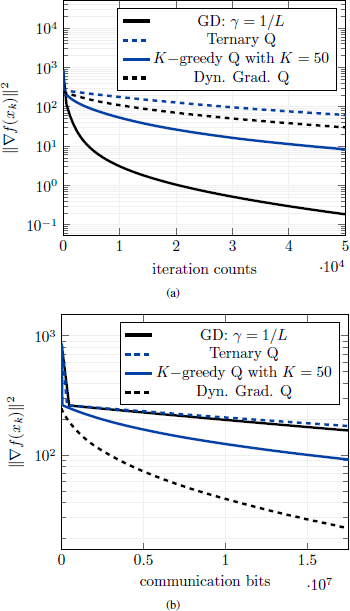
\includegraphics[scale=0.38]{fig.png}
\end{center}


\end{frame}

\begin{frame}
\frametitle{References}
\begin{itemize}
\item {https://ieeexplore.ieee.org/document/8619625}
\item {https://en.wikipedia.org/wiki/Gradient\_descent}
\end{itemize}


\end{frame}
%----------------------------------------------------------------------------------------
%	PRESENTATION SLIDES
%----------------------------------------------------------------------------------------

%------------------------------------------------
%\section{Section 4} % Sections can be created in order to organize your presentation into discrete blocks, all sections and subsections are automatically printed in the table of contents as an overview of the talk
%------------------------------------------------



\end{document}
